% Removed from main.tex on 2026-09-18 (see git history for context).
% Retired experiments: CEM weight scheduling, truth-vs-online geometry precursor,
% legacy full-flow visualization, L1-NMPC three-way matrix, release-detector development record.
% Not \input anywhere; kept for a possible journal version.

%%%% ==== 1. CEM learned weight scheduling + geometry precursor (was \iffalse) ====
\iffalse
The following detailed CEM and precursor-geometry development record is retained in the source
for supplementary use but excluded from the focused manuscript.
\subsection{Learned weight scheduling: a negative result}
We pre-register \textbf{settling time} as the primary metric and report \textbf{within-run
paired differences}, never cross-batch absolutes---the M0 baseline itself moves by \SI{0.9}{s}
across sessions and solver configurations, larger than the effect under test.

Neither search yields a transferable gain, and the two fail differently. The absolute-threshold
search descends monotonically in training ($11.05 \rightarrow 9.74$, $-12\%$) yet lands
\emph{level with} M0 on a cell held out in both axes; the $\alpha$-parameterized search does not
descend at all ($10.46 \rightarrow 10.67$) yet wins 6/6 paired repetitions on that same cell.
A descending training curve and a small held-out win are thus each, on their own, uninformative
here.

We therefore test the surviving candidate $\theta^\star$ against M0 in a pre-registered
$2\times2$ factorial separating its two differences---the dimensionless threshold $\alpha$ and
the four rhythm dimensions, which are orthogonal in the implementation. Arms run back-to-back
within each repetition with order rotated by a 4-order Latin square; $n=8$ per cell, geometry
prior at truth, 64 runs, zero divergence.

\begin{table}[tb]
\caption{Paired median differences vs.\ M0 (primary metric: settling; negative favors the
learned schedule; exact Wilcoxon signed-rank).}
\label{tab:learn}
\centering
\begin{tabular}{@{}lcc@{}}
\toprule
contrast & \SI{0.2}{kg} & \SI{0.3}{kg} \\
\midrule
M0 $\rightarrow$ $\alpha$-only & $+0.20$ ($p=.25$) & $+0.15$ ($p=.20$) \\
rhythm-only $\rightarrow$ $\theta^\star$ & $+0.05$ ($p=.74$) & $-0.35$ ($p=.055$) \\
M0 $\rightarrow$ rhythm-only & $+0.00$ ($p=.84$) & $+0.30$ ($p=.25$) \\
$\alpha$-only $\rightarrow$ $\theta^\star$ & $-0.20$ ($p=.25$) & $-0.15$ ($p=.078$) \\
\midrule
\textbf{M0 $\rightarrow \theta^\star$ (total)} & $\mathbf{-0.05}$ ($p=.95$) &
$\mathbf{+0.00}$ ($p=.84$) \\
\bottomrule
\end{tabular}
\end{table}

All ten settling-time tests are non-significant (smallest $p=.055$) and the total effect is a
median of zero at both masses: \textbf{neither factor contributes a measurable gain}. This is
not a power problem---against the effect sizes previously attributed to $\theta^\star$
($-0.64$, $\SI{-0.40}{s}$) and the paired standard deviations measured here (0.407,
\SI{0.311}{s}), Cohen's $d_z$ is 1.57 and 1.29, giving \textbf{97\% and 87\% power} at $n=8$.
Repeating the \{M0, $\theta^\star$\} comparison at the earlier \SI{10}{Hz} solve rate ($n=8$,
32 runs) likewise reproduces no gain (\SI{0.2}{kg}: $\SI{+0.70}{s}$, $\theta^\star$
\emph{slower} and converging within the window in only 5/8 runs; \SI{0.3}{kg}: $\SI{-0.25}{s}$,
$p=.25$), while M0 itself returns to its historical value there (3.83 vs.\ \SI{3.89}{s})---the
apparatus reproduces; $\theta^\star$ does not.

Finally we resolve the one confound in the earlier held-out win: its M0 baseline used a
\SI{0.8}{N} confirmation threshold rather than the deployed \SI{1.5}{N}. A three-arm paired
replication at that same operating point (M0@\SI{1.5}{N}, M0@\SI{0.8}{N}, $\theta^\star$, the
two M0 arms byte-identical but for the threshold; $n=8$, 3-order Latin square, 24 runs, zero
divergence) finds the three \textbf{indistinguishable on settling} ($0.00$, $-0.00$,
\SI{0.00}{s}; all $p\ge.375$), but shows the \SI{0.8}{N} baseline to be the weaker one on the
control layer (pos.\ error peak $\SI{+0.104}{m}$, $p=.031$), with $\theta^\star$'s advantage
over it ($\SI{-0.091}{m}$, $p=.047$) \textbf{vanishing} against the deployed baseline
($\SI{+0.027}{m}$, n.s.). Part of the historical win is therefore attributable to the weaker
baseline rather than to the learned schedule. Confirmation delay orders strictly and
significantly with the threshold across the three arms (1.28, 2.24, \SI{2.43}{s}; 7/0, 7/0,
8/0), confirming the manipulated variable acts---and that it does not convert into a settling
gain.

\textbf{Interpretation and consequence.} $\theta^\star$ is not a \emph{worse} policy but one
statistically indistinguishable from the hand-designed rule. Since a displacement along all
five dimensions at once costs nothing measurable, the objective is evidently \textbf{flat over
a broad neighbourhood} of M0 rather than sharply peaked at a point the search missed---which is
equally why the search could not descend reliably and why little was lost by not descending. On
this task \emph{when} to reweight carries the benefit; \emph{how much} is weakly determined. We
accordingly retain M0 and claim no learned-scheduling contribution. Every quantitative result
used to compare weight schedules, including
Tables~\ref{tab:nosignal} and~\ref{tab:matrix} and the wind ablation use M0 with the historical
\SI{1.5}{N} threshold. The later continuous-interface batch of
Sec.~\ref{sec:autorelease} also uses the M0 rhythm but normalizes its schedule threshold by the
\SI{0.30}{kg} rack envelope, giving \SI{4.4}{N}; it is not part of the learned-policy
comparison. The sole $\theta^\star$ exception is the qualitative legacy visualization of
Fig.~\ref{fig:b5}, recorded before this ablation concluded. The claim's boundary is the tested
schedule family, task, and settling objective; a richer policy class, a different objective,
or an environment admitting common random numbers may behave differently.

\subsection{Ground-truth-free geometry precursor (truth vs.\ online)}
This ablation predates the final first-moment interface. It tests the narrower question of
whether a motor-torque inversion can remove attachment-geometry truth; the deployed method
subsequently moves the same rotational information into the MHE state $s$ and no longer uses
the steady-flight gate of this precursor.
Table~\ref{tab:matrix} (columns truth/online) shows cells differing by
\SIrange{0.02}{0.13}{m} (within noise) with comparable recovery: removing the attachment-truth
dependency costs nothing. The online CoM estimate tracks truth to \SI{<5}{\percent} on the
dominant component over the eccentricity sweep (Fig.~\ref{fig:cxy}). Over a wider paired
grid the \emph{relative} error spans \SIrange{3.7}{13.7}{\percent}, but the \emph{absolute}
error stays at \SIrange{0.47}{0.63}{mm} across all cells: the noise floor is
payload-independent (rotor-speed quantisation in $\tau$; the denominator $T$ is pinned near
hover), so the relative figure is driven by the true $c$ in the denominator rather than by any
loss of estimator quality---consistent with mass-estimate accuracy being identical across
payloads.

\begin{figure}[tb]
\centering
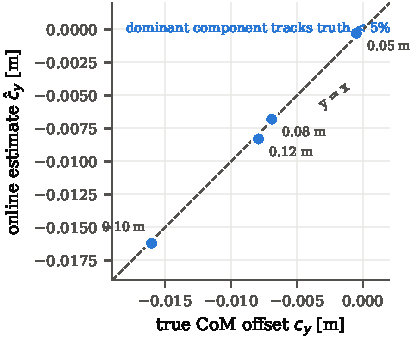
\includegraphics[width=\linewidth]{figs/fig4_cxy_vs_truth.pdf}
\caption{Online CoM-offset estimate vs.\ ground truth across an eccentricity sweep. The
dominant ($c_y$) component tracks truth to $<5\%$ with no attachment measurement---the
estimate uses only motor-speed-reconstructed torques.}
\label{fig:cxy}
\end{figure} \emph{Highlight:} on the hardest cell (\SI{0.3}{kg}/\SI{0.10}{m}) the
truth version diverges 2/5 while the online version is stable 0/5---the divergent truth runs
apply an off-nominal deep grasp instantaneously at full geometry (hover roll torque
\SI{0.459}{N.m} $= \SI{92}{\percent}$ of $\tau_{\max}$), whereas the online version ramps from
a prior. A later paired A/B reproduces this independently (truth $1/8$ vs.\ online $0/8$; the
divergent run was again an outlier grasp at \SI{82}{\percent} of $\tau_{\max}$, while an online
run in the same cell grasped \emph{further} off-centre at \SI{84}{\percent} and completed),
pooling to truth $3/13$ vs.\ online $0/13$.

\emph{Geometry--mass decoupling ablation.} Low stress: decoupled 15/15 no droop vs.\ coupled
10/15 (droop rate $33\% \to 0\%$)---the reproducible evidence for decoupling. We also probed a
high-stress regime ($m_{\min}=1.0$, allowing the mass estimate room to collapse toward the
lower bound) with per-run manifests ($n=16$ per group): here \emph{both} paths were stable
($0/16$ divergence each), and the coupled estimate never actually probed the collapse regime
(minimum $\hat m = 2.03$, all runs converging near truth). An earlier un-logged observation of
coupled-path divergence traced to \emph{off-nominal deep grasps} (attachment depth outliers
near the torque-saturation boundary), an attach-depth artifact rather than a systematic
coupled-vs-decoupled effect at nominal conditions; we therefore rest the ablation on the
low-stress droop result and the bootstrap-decoupling mechanism, not on a divergence-rate
difference.

\fi

%%%% ==== 2. Legacy full-flow visualization (was \iffalse) ====
\iffalse
\subsection{Legacy full-flow visualization}
Figure~\ref{fig:b5} is retained as a qualitative visualization of the physical
grasp--carry--release sequence. It was recorded before the final continuous $m/s/J$ interface
and therefore does not carry the eventless-interface claim of
Sec.~\ref{sec:autorelease}. In that legacy run, a figure-eight carrying an eccentric
\SI{0.3}{kg} load achieved \SIrange{1}{3}{cm} loaded tracking, a release-transient peak of
\SI{0.21}{m}, ${\sim}\SI{2.5}{s}$ recovery, and zero divergence.

\begin{figure}[tb]
\centering
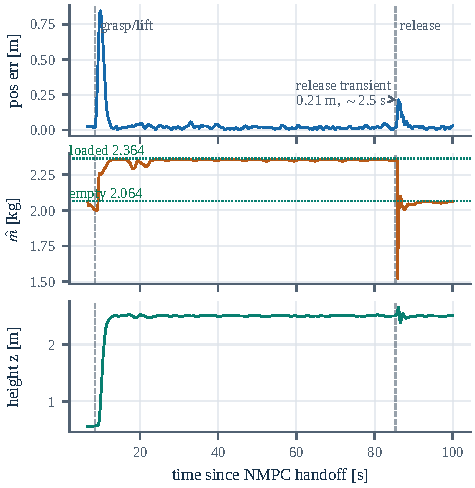
\includegraphics[width=\linewidth]{figs/fig5_b5_fullflow.pdf}
\caption{Legacy complete grasp $\rightarrow$ carry $\rightarrow$ release visualization
(dense $10$\,Hz telemetry throughout). The mass estimate tracks \emph{both} transitions---rising to the
loaded value ($2.364$~kg) at grasp and returning to empty ($2.064$~kg) at release---and the
release transient (position-error peak $0.21$~m, ${\sim}2.5$~s recovery) is fully captured.
This run predates and does not validate the final eventless $m/s/J$ interface; that claim uses
the eventless cohort in Sec.~\ref{sec:autorelease}.}
\label{fig:b5}
\end{figure}
\fi

%%%% ==== 3. L1-NMPC three-way matrix (was live in the PDF) ====
\subsection{Baselines and ablations}
\textbf{L1-NMPC three-way matrix (Table~\ref{tab:matrix}).} \{truth, online, l1\} $\times$
\{0.2, 0.3\}~kg $\times$ \{0.05, 0.10\}~m, $n=5$, 60/60 runs stable, zero divergence. (i)
Within-cell transient peaks agree to \SI{0.05}{m}; L1 is higher in the two low-eccentricity
cells ($p=.008$, $.012$ uncorrected, not surviving correction over eight tests), so we claim
\emph{no} transient advantage. (ii) Against the deployed \emph{online} estimate, \textbf{L1 recovers
\SIrange{8}{32}{\percent} slower} (median \SI{16}{\percent}; significant in three of four
cells); the mechanism is that its compensation low-pass cutoff
$\omega_c$ is bounded by closed-loop stability (0.5 stable, 1.0 unstable on this platform), a
bandwidth wall that explicit estimation does not face. (iii) L1 yields no interpretable
$m$/$c_{xy}$ and still requires the same class prior for gain scaling; it is a translational
3-DoF augmentation driven by $T_{\text{phys}}$ (the commanded thrust self-excites). The larger
\emph{truth} peak in cell 0.3/0.10 is not explained; more accurate parameters need not reduce a
transient peak. All three arms used the earlier mass-only MHE.

\begin{table}[tb]
\caption{Three-way method $\times$ scenario matrix ($n=5$): pos\_err peak~[m] / recovery~[s].}
\label{tab:matrix}
\centering
\begin{tabular}{@{}lccc@{}}
\toprule
cell (mass/ecc) & truth & online & l1 \\
\midrule
0.2 / 0.05 & 0.806 / 4.28 & 0.768 / 3.70 & 0.821 / 4.26 \\
0.2 / 0.10 & 0.794 / 3.62 & 0.810 / 3.92 & 0.812 / 4.24 \\
0.3 / 0.05 & 0.834 / 3.56 & 0.837 / 3.72 & 0.883 / 4.90 \\
0.3 / 0.10 & 1.011 / 3.64 & 0.876 / 3.88 & 0.891 / 4.54 \\
\bottomrule
\end{tabular}
\end{table}


%%%% ==== 4. Release-detector development record (was \iffalse) ====
\iffalse
and the 21/21 paired result demonstrates that its output can drive the complete NMPC recovery
without a drop event. It does not establish detector robustness: historical replay still misses
14/72 releases, and the 95\% interval from 21 successes permits a true failure rate near
16\%. The key structural issue in the audited profile was that its shared \SI{4.4}{N} residual
threshold was chosen to suppress the residual path for a \SI{0.30}{kg} envelope study, but the smallest supported
\SI{0.15}{kg} payload produces only a \SI{1.47}{N} weight step. Lowering that shared threshold
would also change MHE weight scheduling and would confound earlier ablations. The subsequent
release-only detector solved that coupling but its fastA branch failed the randomized smoke:
3/9 flights released the estimator state prematurely. In loaded figure-eight flight, payload
mass had a fifth percentile of \SI{-0.1032}{kg} relative to the bare airframe and remained below
the nominal empty threshold for a median \SI{14}{s} (maximum \SI{48}{s}); quantity is therefore
not valid evidence in that regime. Adding a lower-bound exclusion still leaves 13.6\% of loaded
frames below threshold, while a weak moment gate has not been distributionally justified.
We consequently reject fastA and retain only moment-gated paths. If they time out, the controller
must enter a conservative hover/land abort while keeping the payload state unresolved; timeout
must not clear the model or reset adaptive state. This accepts a possible missed release under
the synthetic $\rho=1.52$ cross-boundary stress case rather than retaining a path with an
observed one-third flight-level false-release rate. A post-removal replay flagged one apparent
slow-path false release in run~152924, but that record is not a valid clean counterfactual: it was
generated after the old fastA branch had already cleared and re-armed the online lifecycle.
Nevertheless, it exposes a real upstream defect. Five consecutive MHE failures triggered a
re-anchor that explicitly set $\hat s=0$, and the release counters consumed that invalid value
before a fresh successful solve. The appropriate correction is health/freshness gating and
counter reset on solve failure or re-anchor, not a post-hoc lower ratio cutoff. This correction
was then exercised in 12 clean online flights: none released before the command, 11/12 obtained
valid late evidence (median detector delay \SI{1.9}{s}), and the remaining flight stayed unresolved
without clearing the model. Three flights crossed the \SI{12}{s} unresolved timeout and two later
recovered when delayed evidence arrived.

A coverage gap in that smoke was subsequently corrected: the unified detector had remained
nested under a legacy mass-arm latch, so one autonomously detected attachment never entered the
moment decision. Commit \texttt{ddfe9d2} moved the unified detector under the autonomous load
latch plus health while leaving the mass-arm local to the legacy mass-only branch. The first four
post-fix flights then exposed a different pre-existing issue and were stopped before acceptance:
the running maximum used as the loaded-moment reference absorbs figure-eight estimation errors.
Samples beyond the simulation envelope $m_{p,\max}r_{xy,\max}=\SI{0.039}{kg.m}$ occur in both the
old data (49/644 frames, 7.6\%, four of 11 flights) and the post-fix data (49/268, 18.3\%, three of four
flights), beginning about \SIrange{26}{28}{s} after attachment in the dynamic segment. Thus the
gate change increased exposure but did not create the estimator error. A safe revision must build
a robust loaded-moment reference from an autonomously identified low-dynamic, healthy,
in-envelope window, freeze it before dynamic flight, and treat out-of-envelope samples as invalid
evidence and an estimator-quality diagnostic. Raw $\hat s$ may also fail to return to zero after a
real drop; this remains a safe miss handled by \textsc{unresolved}, not permission to clear $s$
from the controller's command.
\fi
